\documentclass[acmtog, authorversion]{acmart}

\usepackage{booktabs} % For formal tables

% TOG prefers author-name bib system with square brackets
\citestyle{acmauthoryear}
\setcitestyle{square}


\usepackage[ruled]{algorithm2e} % For algorithms

\usepackage{hyperref}
\usepackage{float}

% Metadata Information
\acmJournal{TOG}
\acmVolume{1}
\acmNumber{1}
\acmArticle{1}
\acmYear{2018}
\acmMonth{12}

% Copyright
%\setcopyright{acmcopyright}
%\setcopyright{acmlicensed}
%\setcopyright{rightsretained}
%\setcopyright{usgov}
\setcopyright{usgovmixed}
%\setcopyright{cagov}
%\setcopyright{cagovmixed}

% DOI
\acmDOI{0000001.0000001_2}


% Document starts
\begin{document}
% Title portion
\title{Music Genre Classification Using Time-Frequency Representation}

\author{Chenyang Yu}
\affiliation{%
  \institution{University Of California, Riverside}
  \streetaddress{862052273}
  }
\email{cyu059@ucr.edu}
\author{Irem Ergun}
\affiliation{%
  \institution{University of California, Riverside}
  \city{862051254}
}
\email{iergu001@ucr.edu}
\author{Nikhil Gowda}
\affiliation{%
 \institution{University of California, Riverside}
 \streetaddress{861172066}
 }
\email{nikhilgowda@gmail.com}


\renewcommand\shortauthors{Yang C. et al}

\begin{abstract}
  More and more web applications and music streaming services count on automated music genre classification (AMGC). Therefore, it is important to achieve 
  genre classification tasks accurately. This is also an interesting task because there are many approaches that can be taken to extract the features and 
  do the classification, and, yet there is not a single method that significantly outperforms the others since the data is immensely varied and not usually
   labeled properly. Hence, there is still ongoing research about this topic, leading this task to be open-ended and suitable for further development. We 
    took different approaches in feature extraction and classification and compare our results to be a part of this pursuit of implementing a 
   successful classifier for music genre classification. More specifically, given GTZAN genre collection data, we used K-nearest neighbors, 
   convolutional neural networks and decision tree algorithms in order to classify genres of different songs. We evaluated our results experimentally and 
   achieved a promising accuracy.
\end{abstract}
\keywords{Music genre classification, spectrogram,
convolutional neural networks, kNN, decision trees}



\maketitle
\section{Introduction}
New songs are released by several artists every day and music steaming services integrate those songs to their databases. Since music recommendation systems
are on the rise, it is crucial to label them according to their genres. Doing this manually is a tedious job considering the amount of data. Therefore, automated
music genre classification is an important problem and it has been studied extensively in the literature after \cite{tzanetakis2002musical}.
However, even though many different approaches were implemented to solve this problem, none of them significantly outperforms the others and this remains an
open problem. The complexity of the problem arises due to the vastness and variety of data along with the fact that there are many genres. \\
Considering the importance and the complexity of the problem, we are motivated to work on the music genre classification problem. Finding the appropriate dataset for this problem is the first step of our roadmap. 
Since we want to achieve the task of classifying music using the audio files, we used the GTZAN dataset\footnote{\url{http://marsyasweb.appspot.com/download/data_sets/}}, which consists of 1000 audio files from 10 different
genres. The labels in the dataset are blues, classical, country, disco, hip hop, jazz, metal, pop, reggae and rock. Each genre has 100 songs, each of them are 
30 seconds long. \\
Feature extraction is an important part of the problem since many different features can be extracted using audio signals of the songs.  
Considering all the work done on feature extraction from audio files, which will be described further in Section 2, we decided to proceed with 
time-frequency features of the songs, which consist of Tempo, Pitch, Tune, Pitch, Spectrograms, etc... Tempo refers to average beats of the whole audio file, it use BPM (Beat per minute) as unit. We use Mel-frequency cepstral coefficients (MFCC) to capture the tune feature and represented as a time series data. The constant-Q transform (CQT) of an audio signal may represent the pitch feature of the audio file. The time series constant-Q power spectrum data is used as the feature. Spectrograms represent the strength of a signal given a specific time and a frequency. The spectrogram of an audio signal is calculated
by taking short time Fourier transform of a time window extracted from the signal.\\
Having time-frequency features in our hands, we decided to implement three different classifiers. The first one is k-NN. This is one of the most representative Lazy Learning Classifications. For the given training data with labels, the prediction of testing tests will be made depending on the distance between testing data entity and the k-nearest training data entity. \\
The second classifier we implemented was decision trees. Decision trees are known to be optimal for binary classification but applying them to a large classification problem such as a 10-level one is still quite possible and has been applied before to complex problems. We used a binary classification tree similar to CART and used the Gini index for potential splits. The idea here is to reduce entropy at each level to make sure our splits do not break up individual classes to a high degree, this has to be done weighting each class as a contributing factor to the split. This potential splitting can be terminated by either a maximum number of nodes reached in which case we ensure to make the last level of the tree leaf nodes, or the case of max tree depth in which case at a specified depth, there exists only leaf nodes (the actual chosen classification). With this approach we can use features such as tempo, or more complex 2d-array features such as MFCC (Mel Frequency Cepestral Coefficients). 
Our third classifier was convolutional neural networks. Convolutional neural networks are commonly used in image classification tasks. To be able to do that, 
we constructed images using spectrograms extracted from the audio files. After some preprocessing, images are fed to the convolutional neural network. 
To the best of our knowledge, we are the first ones to try convolutional neural networks that was not pre-trained before to tackle this problem.\\
The organization of our report is as follows. Section 2 includes the literature review we have done. In Section 3, we describe out methodology for each method
we implemented. Section 4 compares the results we gathered from different methods and gives a discussion. Section 5 concludes the paper while also talking about
the future work.
\section{Related Work}
Since we wanted to extract the most useful features for our task, we explored papers about feature extraction and feature selection. \cite{wyse2017audio} 
is mostly concerned different ways to extract features from audio files because it explains the intuition behind the choice of spectrogram images. 
It describes some experiments done with Mel Frequency Cepstral Coefficients (MFCCs) and points out that their accuracy is low because MFCCs are lossy 
representation of audio files. The paper indicates that raw audio files are lossless and trivial to convertible to audio. However, this approach is slow. 
Another approach might be to use the magnitude spectra. Recent research made this possible by implementing fast algorithms to calculate the spectra. 
Spectrograms include the spectra, time and frequency information of an audio signal. Hence, as the paper indicates, “This representation is thus at least 
suggestive that some of the convolutional neural network architectures for images could be applied directly to sound.” After giving this remark, the paper 
describes some possible CNN implementations and tunings for achieving a classification task using audio files. The conclusion of the paper indicates that 
using spectrograms and CNNs for audio related classification tasks is a good direction in research as the data has fewer dimensions compared to raw audio 
and entails more information compared to many other features extracted from audio files. This result indicates that using spectrograms and CNNs for music 
genre classification could be an interesting approach, even though the paper was not directly about genre classification problem. The paper lacks a proper 
demonstration of the results they yielded and is not very specific about the experiment setup. This could be improved by doing proper experiments and 
clearly explaining the results after the experiments with genre classification are completed.
Next, we scanned the literature for papers which use the similar approach to ours. \cite{bahuleyan2018music} extends 
the work described in \cite{wyse2017audio}. The authors use two different feature sets, 
one of the feature sets is spectrogram images and the other set is hand-crafted time and frequency domain features, such as tempo, MFCC, chroma features, 
et cetera. The authors use the pre-trained weights from VGG-16 \cite{simonyan2014very} and they use transfer learning to achieve classification using spectrogram images and logistic regression, random forest, gradient boosting and 
support vector machines to achieve classification using hand-crafted features. They try different combinations of implemented methods and compare results.
 Accuracy, F-score and AUC are used as evaluation metrics for the comparison of results. Results indicate that the most important hand-crafted feature for
  this tasks is MFCCs, using a combination of time and frequency domain features yielded better results than using only time or only frequency domain 
  features alone, and the best classification method is CNNs which are using spectrogram images as features. This paper explains each step in the experiment
   setup clearly, giving detailed results and analysis. Running an actual convolutional neural network on spectrogram images is our contribution to this work.
   Also, in the dataset, we have 10 genres, which is more than \cite{bahuleyan2018music} has.\\
KNN Model-Based Approach in Classification \cite{Guo2003knn}: One of the most representative lazy classification. The prediction is made by the majority 
voting of its nearest neighbors, which means we could save the time for training. As long as we list the features for each data point, KNN classification 
is rather easy to implement. Even if we are facing the continuous feature like MFCC, we can setup the sample rate and use Dynamic Time Warping(DTW)\cite{tang2010dtw} to calculate the distance of two series data. The accuracy and precision are also good when there is enough representative data points. On the other side, 
we risk at taking more time on verifying procedure (Compare with other model-based learning). When the amount of data points is large, finding the 
nearest neighbor may become a complex problem. Also, how to choose a good k value and a good distance calculation function may also be complicated. A bad 
choice may compromise the final accuracy.
In terms of implement algorithm, we don’t really need to calculate all distance and pick k-nearest. Instead, we can use k-d tree to reduce the time 
complexity. Also, we expect the choice of k value will affect the accuracy and we will run several times under different k value to test. As the result, 
we will build a table to store k’ neighbor neighbor for each data points (where k’ is larger than the maximum k value we are going to try). Although this 
approach significantly increase the space complexity, the time complexity can be also significantly reduced. \\
The feature selection method was \cite{tang2014feature}. When we use the KNN-classification, the cost of 
computational time may be a serious problem. It is caused by the calculation of distance, which is proportional the the dimension of our feature space 
(In other word, the number of features). If we can find a efficiency approach to eliminate the irrelevant features, we can reduce the computational time 
and improve our prediction at the same time. 
Forward selection and backward elimination are two of the most common selection approaches. By building a search tree, the height of each level represents 
the size of selection feature. Expands the node to next level until all features are included. The overall maximal accuracy combination is our final 
choice. Since the complete tree will need O(n!) expanding node (for n feature in the beginning), it is more realistic to use greedy strategy to build the 
tree (For each level, choose the maximal accuracy in that level to expand). The expanding nodes is $O(n^2)$. Although it increases the overhead to finish 
the prediction, reducing the irrelevant feature also helps to explain the result of classification.\\ 
From Precision, Recall and F-Factor to ROC, Informedness, Markedness, and Correlation[6] we cab make ab assumption that Precision, 
Recall and F-factor all contain a bias, if not understood properly, can falsely represent conclusions in data, especially in the handling of negative 
outcomes. Without knowledge of informedness or markedness (and also a special attention to chance), examination of results often overlook important 
elements such as positive negatives (Jaccard’s also does not account for this). In the article, Informedness, is defined as a way to quantify how 
informed a predictor is (Recall + Inverse Recall - 1) and Markedness, is defined respectively as how marked a predictor is for a given condition 
(Precision + Inverse Precision - 1). We can use this discussion to see Recall evaluation as reflecting the bias but removing weight in Informedness as 
well as Precision reflecting prevalence and removing weight in Markedness. Methods such as Kappa have been better relationships with Informedness and 
Correlation. The paper goes on specifying and proving this discussion graphically and argumentatively (i.e. many terms are borrowed from Psychology not 
properly applicable to data science). With proper considerations, our formed contingency matrices that are dichotomous or mutually exclusive 
(multi-class), are far less biased than Precision and Recall methods. Further direct relationships in Informedness, Markedness, and Matthew’s Correlation 
with consideration in biased/unbiased and high/low degree of freedom all account for better confidence intervals when looking at our completed data. This 
is directly applicable to our project in how we decide to classify our data to enhance to escape basic Recall and Precision tests. 
A Survey on Decision Tree Algorithm For Classification[7] shows how decision Trees have strong characteristics in speed and learnability, they can 
be limited for example by value choice (higher values are used mostly) and over-classification (leading to inaccuracy). CHID’s approach can handle missing 
values but has limited pruning capacity. CART’s approach can produce classification or regression trees and pruning but has only binary splitting. ID3’s 
approach reduces the number of dividing classifications significantly and so forth. In addition to what exists, there is software that integrated decision 
tree algorithms in a more efficient manner such as GAtree harnessing genetic algorithms to further evolve trees or OCI that can efficiently build nodes 
based on the linear combination of continuous features. The current troubles of decision trees are enumerated with things such as the fragmentation 
problem (unnecessary fragmentation when many features being tested) or replication problems (when a subtree contains its own subtree). Or specifically, 
when creating an ID3, without backtracking an optimal decision can be made locally but not globally. Also, decision trees cannot handle certain structures 
efficiently such as XOR or multiplexer problems without being extremely large decision trees. In addition, information gain can pose a problem since 
multi-variable values will be valued possibly creating a wrong classifier. The current state of decision trees is to incorporate in their algorithms, 
a way to handle such problems. Concerning these two paper's relation, we can use a sense of proper informativeness when we use our Gini index to reduce as much entropy as possible. There stands a relationship between these two concepts, Gini index being a form of informativeness. Building a decision tree than could be seen as a level to level entropy reduction is a deciding complex factor in multi-label classification where entropy may still seem large after a single binary split. Hence, our definition of informativeness can be changed regarding this information. Information gain should be judged more strongly after at least after 3 levels of splits for a 10 level classification (8 labels can be classified). This influences how we built the decision tree, mainly ensuring the level of tree was apt for finding a proper test for information gain and likewise, entropy reduction. 
\section{Proposed Method}
We propose three different methods to tackle this problem and describe them in detail throughout this section.
\subsection{k-NN}
Our prediction will be made through the k-nearest neighbors. The distance between two entity will be calculate by Lp-norm and Dynamic time wrapping(as Figures below). Since usually not all k-nearest neighbors will be the same label, we will use majority labelling of neighbor in that case. 
\begin{figure}[h!]
  \centering
  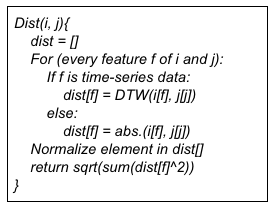
\includegraphics[width=0.2\textwidth]{dist}
  \caption{How to calculate the distance between 2 entity}
  \end{figure}
\begin{figure}[h!]
  \centering
  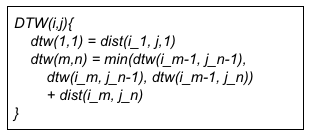
\includegraphics[width=0.2\textwidth]{dtw}
  \caption{Use Dynamic time wrapping to calculate the similarity between 2 time-series data}
  \end{figure}
\\Since the choice of k-value will significantly affect the performance, we will compare the accuracy between different k-values. One of the disadvantages of k-NN is that when dealing with too many features (causing high dimension space), the cost of calculating distance will significantly raise. Also, the effect from outliers will also rise and pose a risk. We reduce the irrelevant feature by feature selection algorithm.
\begin{figure}[h!]
  \centering
  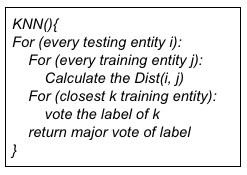
\includegraphics[width=0.2\textwidth]{knn}
  \caption{Algorithm of k-NN}
  \end{figure}
  
\subsection{Decision Tree}
Decision trees are arguably the easiest decision streams to visualize. Each node split represents a binary decision (for binary classification trees) for information gain which can be seen as a greedy approach. At which node split point (assuming continuous data), would we gain the most information from? This question defines us creating new node levels. But first, you propose a feature extraction, each done individually by us. We used libROSA, a popular feature extractor/ audio visualizer for raw audio files. Using our dataset, we can load files one by into a script, in my case, a Python script. Extracting features one by one, we can specify single scalar results or 2d array results (e.g. tempo vs MFCC), into our data set. Our dataset also can have a rank attribute in its right-most column for each object to represent the class it is part of (e.g. Rock or Country). From then, we can feed our data set into our multi-label decision tree.
\begin{figure}[h!]
  \centering
  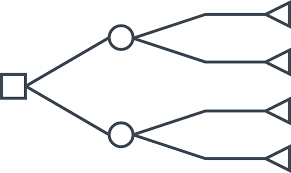
\includegraphics[width=0.5\textwidth]{decisiontree.png}
  \caption{A binary decision tree}
  \end{figure}

We can start off with a basic set of different attributes each making up different ranges of continuous data. Our Gini index will mark our potential split at the 2nd level. This split is dependent on most information gain, as in the classes represented in each split minimize class randomness in each specific group. The Gini index holds from a value of 0->1 (0 meaning complete equality, 1 meaning complete inequality). Running the algorithm, the tree is grown through the gini index and is terminated by a specific level of the tree or specific number of nodes created. We make sure we have a special check for our rank from 0->9 representing each class. After the tree is constructed, we have a prediction function that can be specified to have 10-fold cross-validation to test our accuracy. This approach, not considering any extensions such as pruning or maybe a more popular approach of random forest techniques, received an 8\% better than chance accuracy. 

\subsection{Convolutional Neural Network}
Convolutional neural networks are mostly used for image classification tasks. To make them applicable to our problem, we constructed spectrogram images using
Python Librosa library\footnote{\url{https://librosa.github.io/librosa/}}. The sampling rate used for Fourier transform is the native sampling rate of the 
audio file. The images are saved as PNG files. At this stage, we examined spectrograms of the songs belonging to different genres and tried to understand 
whether the differences are easily noticeable. An example comparison is given in Figure 1. This example demonstrates the fact that the differences between spectrograms are even visible to the eye, which is a very promising preliminary result for 
our method.\\
\begin{figure}[h!]
  \centering
  \includegraphics[width=0.5\textwidth]{comparison_spectrogram}
  \caption{spectrogram of a disco song (left) and a metal song (right)}
  \end{figure}

After the images are saved, they are read as RGB images. Since the images are used in our method are all from the same color scale, 
the color scale would not affect our classification. The dimension of the resulting images are 324x900x3. \\
As the dataset is scarce, some data augmentation techniques are required. For this purpose, all images are split into threes in the time domain, resulting in 
input matrices having dimensions as 324x300x3. All data points are combined in one matrix having dimensions 3000x324x300x3. Finally, that matrix is normalized
using z-normalization, which includes subtracting the mean from each data point and then, dividing them by the standard deviation. This concludes the feature
extraction part of our method.\\
The next step is to construct the the architecture for the neural network. For that purpose, Keras library is used \footnote{\url{https://keras.io}}. Since
our dataset is small, a simple neural network architecture is considered. An architecture similar to Le-Net5 \cite{lecun2015lenet} is constructed.
 Some dropout layers are added to prevent overfitting. The architecture of the network is given in Figure 2. \\
\begin{figure}[h!]
  \centering
  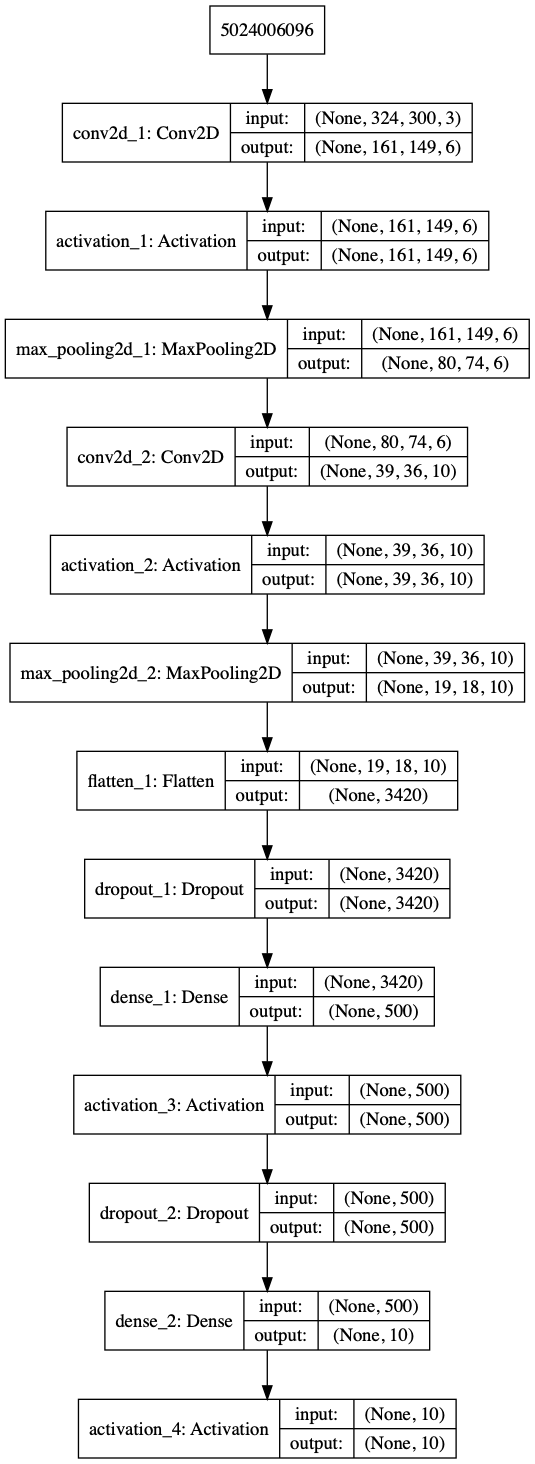
\includegraphics[width=0.25\textwidth]{model.png}
  \caption{CNN architecture}
  \end{figure}

Hyper-parameters are tuned via experimentation. The model has two convolutional layers and they are both followed by activation and pooling layers. The first layer has 6 filters, having 4x4 size. This is selected using the 
equation $W=(W_{input}-F_{w}+2P)/S+1$ ,W: activation map width, $W_{input}$: input width, $F_{w}$: filter width, P: padding, S: stride (Same formula applies
to activation map height if we replace the widths with heights), which gives the size of the activation map. We selected those parameters in a way that 
the size of the activation map would be reasonable. The padding size is 2x2. 
The second convolutional layer has the same filter size but has more (10) filters because the deeper layers represent more detailed features of the dataset.  The activation 
layer that follows the convolutional layers is a RELU activation layer and the pooling layer has 2x2 pool size 2x2 strides, which is the most common pooling 
layer type in the literature. Then, the input is flattened and converted to a vector to be used for the next stages.\\
The next part of the architecture consists of two groups of layers. Each group has a dropout layer, a fully connected layer and an activation layer.
Dropout layers are added for preventing overfitting and their rates are 0.1. First fully connected layer has 500 units whereas the second one has 10 units, which
is equal to the number of classes. The first activation layer uses RELU whereas the second one is softmax because we are doing classification.\\
Rest of the parameters of the network are found via experimentation. The number of epochs are 10 and the batch size is 64. The weights of the network are 
initialized randomly and the Adam, which is described in \cite{kingma2014adam} is used for updating the weights and learning rate is 0.001. \\
\section{Experimental Evaluation}
For comparing the accuracy of our methods, we used 10-fold cross validation. We randomly split the dataset into train and test data, with a ratio of 9:1
and fed the dataset to our algorithms. The confusion matrix for the convolutional neural network approach is given in Figure 3. The mapping of the labels is as follows:
 0: Metal, 1: Pop, 2: Disco, 3: Blues, 4: Classical, 5: Reggae, 6: Rock, 7: Hip-hop, 8: Country, 9: Jazz. The accuracy for CNN is 69\%. \\
\begin{figure}[h!]
  \centering
  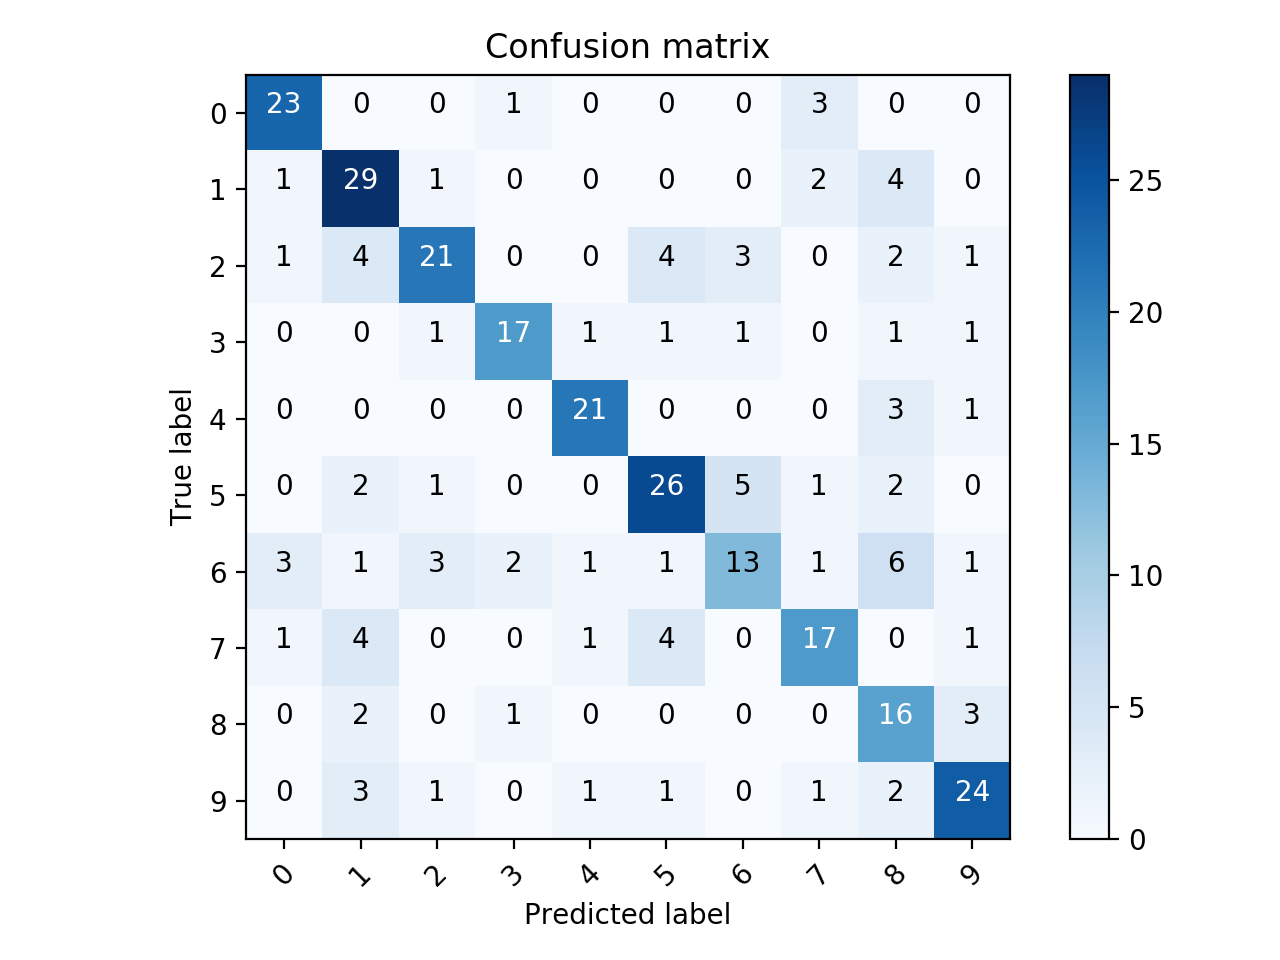
\includegraphics[width=0.5\textwidth]{conf_matrix}
  \caption{Confusion matrix for convolutional neural network approach}
  \end{figure}
\\
For k-NN classification, we test the accuracy under different k-value. As we can see from the below figure, the accuracy is rather low when value is small. The knee region is found in k=10, After that, the accuracy is increased but not so obviously.

\begin{figure}[h!]
  \centering
  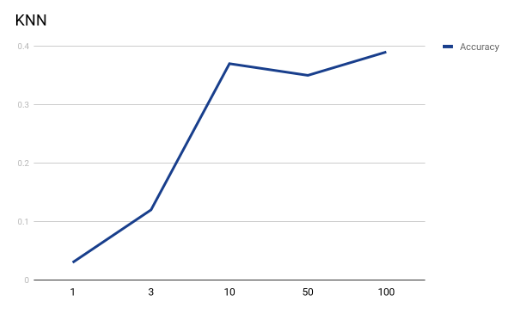
\includegraphics[width=0.5\textwidth]{knnAccuracy.png}
  \caption{Accyracu of k-NNN under different k-value}
  \end{figure}
\\  
For the decision tree, we can see an accuracy of 18\% with the highest accuracy being in discerning Classical and Pop with the worst Rock and Metal. Doing pre-liminary tests, binary classifcation was ~100\% amongst two separate genres such as Pop and Jazz. See Fig. 9.

\begin{figure}[h!]
  \centering
  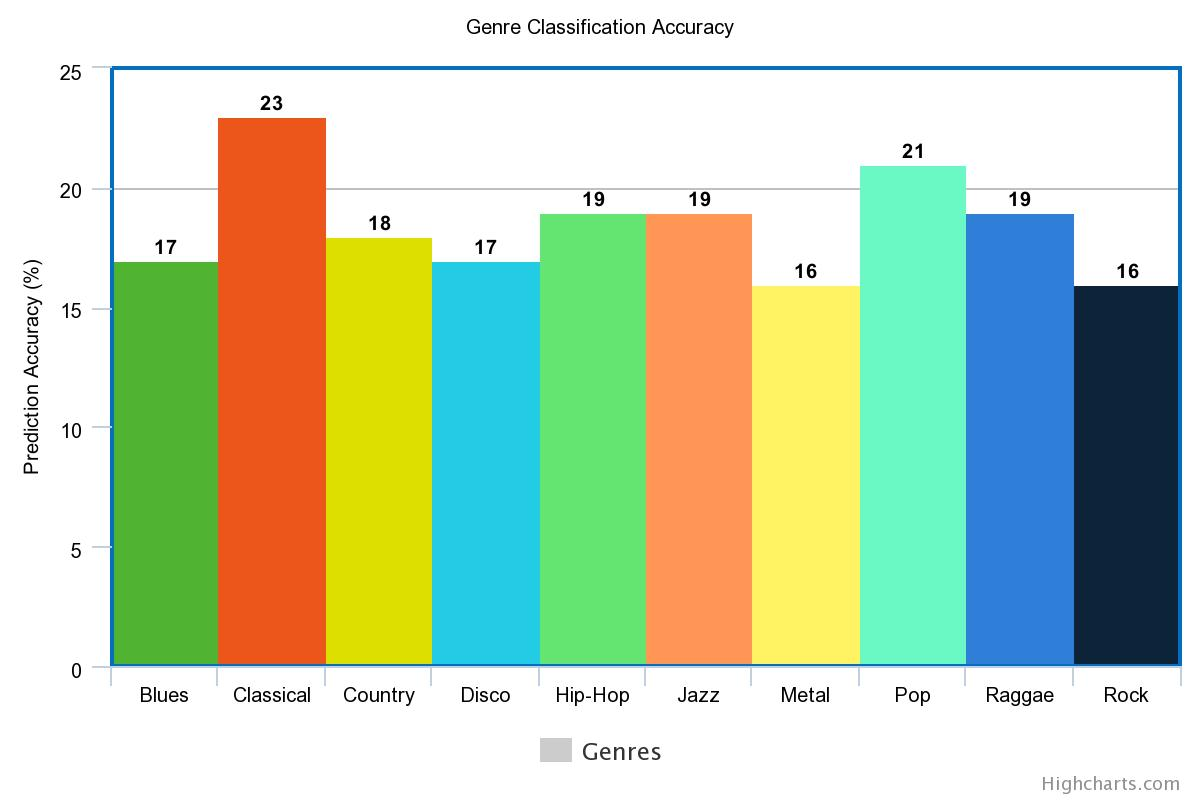
\includegraphics[width=0.5\textwidth]{meta-chart.jpeg}
  \caption{Accuracy Among Genres for Decision Tree}
  \end{figure}


Lastly, we compare the results of different methods. The comparison is summarized in Table 1.
\begin{center}
  \captionof{table}{Comparison of accuracies of different methods} \label{tab:title} 
  \begin{tabular}{ |c|c| } 
   \hline
   Method & Accuracy  \\ 
   k-NN & 37\% \\ 
   Decision tree & 18\%  \\ 
   CNN & 70\% \\
   \hline
  \end{tabular}
  \end{center}
Convolutional neural network seem to outperform the other methods.
\section{Discussion and Conclusion}
Music genre classification is a very important and challenging task. We used time-frequency features of the audio files to tackle this problem. We implemented
k-NN, decision trees and neural networks and compared their performance. Convolutional neural networks seem to outperform the other methods.
 Moreover, our results were promising in general since our accuracy was almost at least two times the random even for our classifier with lowest accuracy and with our highest performing method, we got 70$\%$ accuracy, which is seven
times better than random. Even though the dataset was small to run on neural networks, we got good results compared to many other studies in the literature. \cite{mckay2004issues} \\
Based on the results, for future work, we plan to collect more data to prevent overfitting. Due to the scarcity of the dataset, we could not try complex
neural networks. After collecting more data, more complex neural network architectures can be tried for solving this problem . Then, the signal itself can be
preprocessed before extracting some features from it. For example, we want to improve the signal to noise ratio of the signal before processing it by using a pre-emphasis filter. A combination of approaches hold value. For example, regarding binary decisions, pre-liminary tests showed decision trees to be ~100\% accurate between discerning Rock and Jazz. 
We also plan to try chroma features
for k-NN and decision trees as they might yield better results. The spectrograms generated for neural network are composed only of the magnitude of the signal, 
phase information is lost. This lossy representation might affect accuracy in a bad way. Hence, it would make more sense to save the phase information of the signal
in a different matrix and use the magnitude and the phase to make classification. Considering our results, we believe that our approach is very 
useful in tackling this problem and there is plenty of room for further development. 

\bibliography{sample-acmtog}
\bibliographystyle{plain}

\end{document}
